\documentclass[]{article}

\usepackage{graphicx, float}
\usepackage{caption}
\usepackage{subcaption}

\usepackage{amsmath,amsfonts,amsthm,amssymb}
\usepackage[cal=cm]{mathalfa}

\newtheorem{mydef}{Definition}
\newtheorem{myprop}{Property}
\newtheorem{mythm}{Theorem}
\newtheorem{mylem}{Lemma}

\graphicspath{{./Figures/}}

%opening
\title{Penrose Aperiodic Tiling of the Plane and Collin's Walks}
\author{Jesse Bettencourt}

\begin{document}

\maketitle



\section{Introduction}
\subsection{Theory of Periodic Tiling}

In 1619, Kepler discovered the third law of planetary motion which he described in his book \textit{Harmonices Mundi} (The Harmonies of the World). In this work, Kepler also provides the first mathematical treatment of plane tiling by regular polygons. Primarily, he shows that only 3 regular polygons; triangles, squares, and hexagons; are able to completely tile the plane, that is, without overlap or gaps (Fig. \ref{fig:regular}). Further, Kepler experimented with tilings produced by combinations of polygon tiles (Fig. \ref{fig:combo}). While patterns of this kind have been known to the ancients, featured widely in art and architecture, it was Kepler who first provided a mathematical framework with which to discuss these tiling patterns. One aspect of this treatment is the symmetry of the tiling. 

We can describe the tiling patterns generally by the symmetries which they admit. In planar tilings there are four fundamental types of symmetry: 
\begin{enumerate}
\item A tiling has \textbf{rotational} symmetry if it can be rotated a non-trivial angle about a point and overlap itself identically.
\item A tiling has \textbf{reflection} symmetry if it can be mirrored across a line and overlap itself identically. 
\item A tiling has \textbf{translational} symmetry if it can be shifted by some non-trivial distance in a direction and overlap itself identically.
\item A tiling has \textbf{glide} symmetry if it can be translated some distance, then reflected about a line, and overlap itself identically.
\end{enumerate}

Using the notion of translational symmetry, we can introduce a new property of plane tiling, periodicity. A tiling is said to be \textbf{periodic} if it admits translational symmetry. The tilings in Fig. \ref{fig:regular} and Fig. \ref{fig:combo} are all periodic, but is it possible to make a tiling pattern which is not periodic? Well, actually it's quite easy. Consider the square tiling in Fig. \ref{fig:square} but with each column shifted up and down by some random decimal amount. This tiling of jostled squares would completely tile the plane, but since the squares are all randomly shifted there's no way we could translate the entire plane so that it overlaps itself. This is an example of a tiling pattern which does not have the periodic property, we call these patterns aperiodic. 




\begin{figure}
        \centering
        \begin{subfigure}[hb]{0.3\textwidth}
                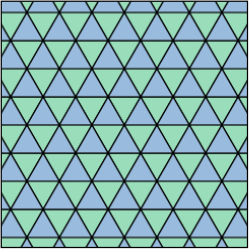
\includegraphics[width=\textwidth]{triangle}
                \caption{Tiling by triangles}
                \label{fig:triangle}
        \end{subfigure}%
        ~ %add desired spacing between images, e. g. ~, \quad, \qquad, \hfill etc.
          %(or a blank line to force the subfigure onto a new line)
        \begin{subfigure}[hb]{0.3\textwidth}
                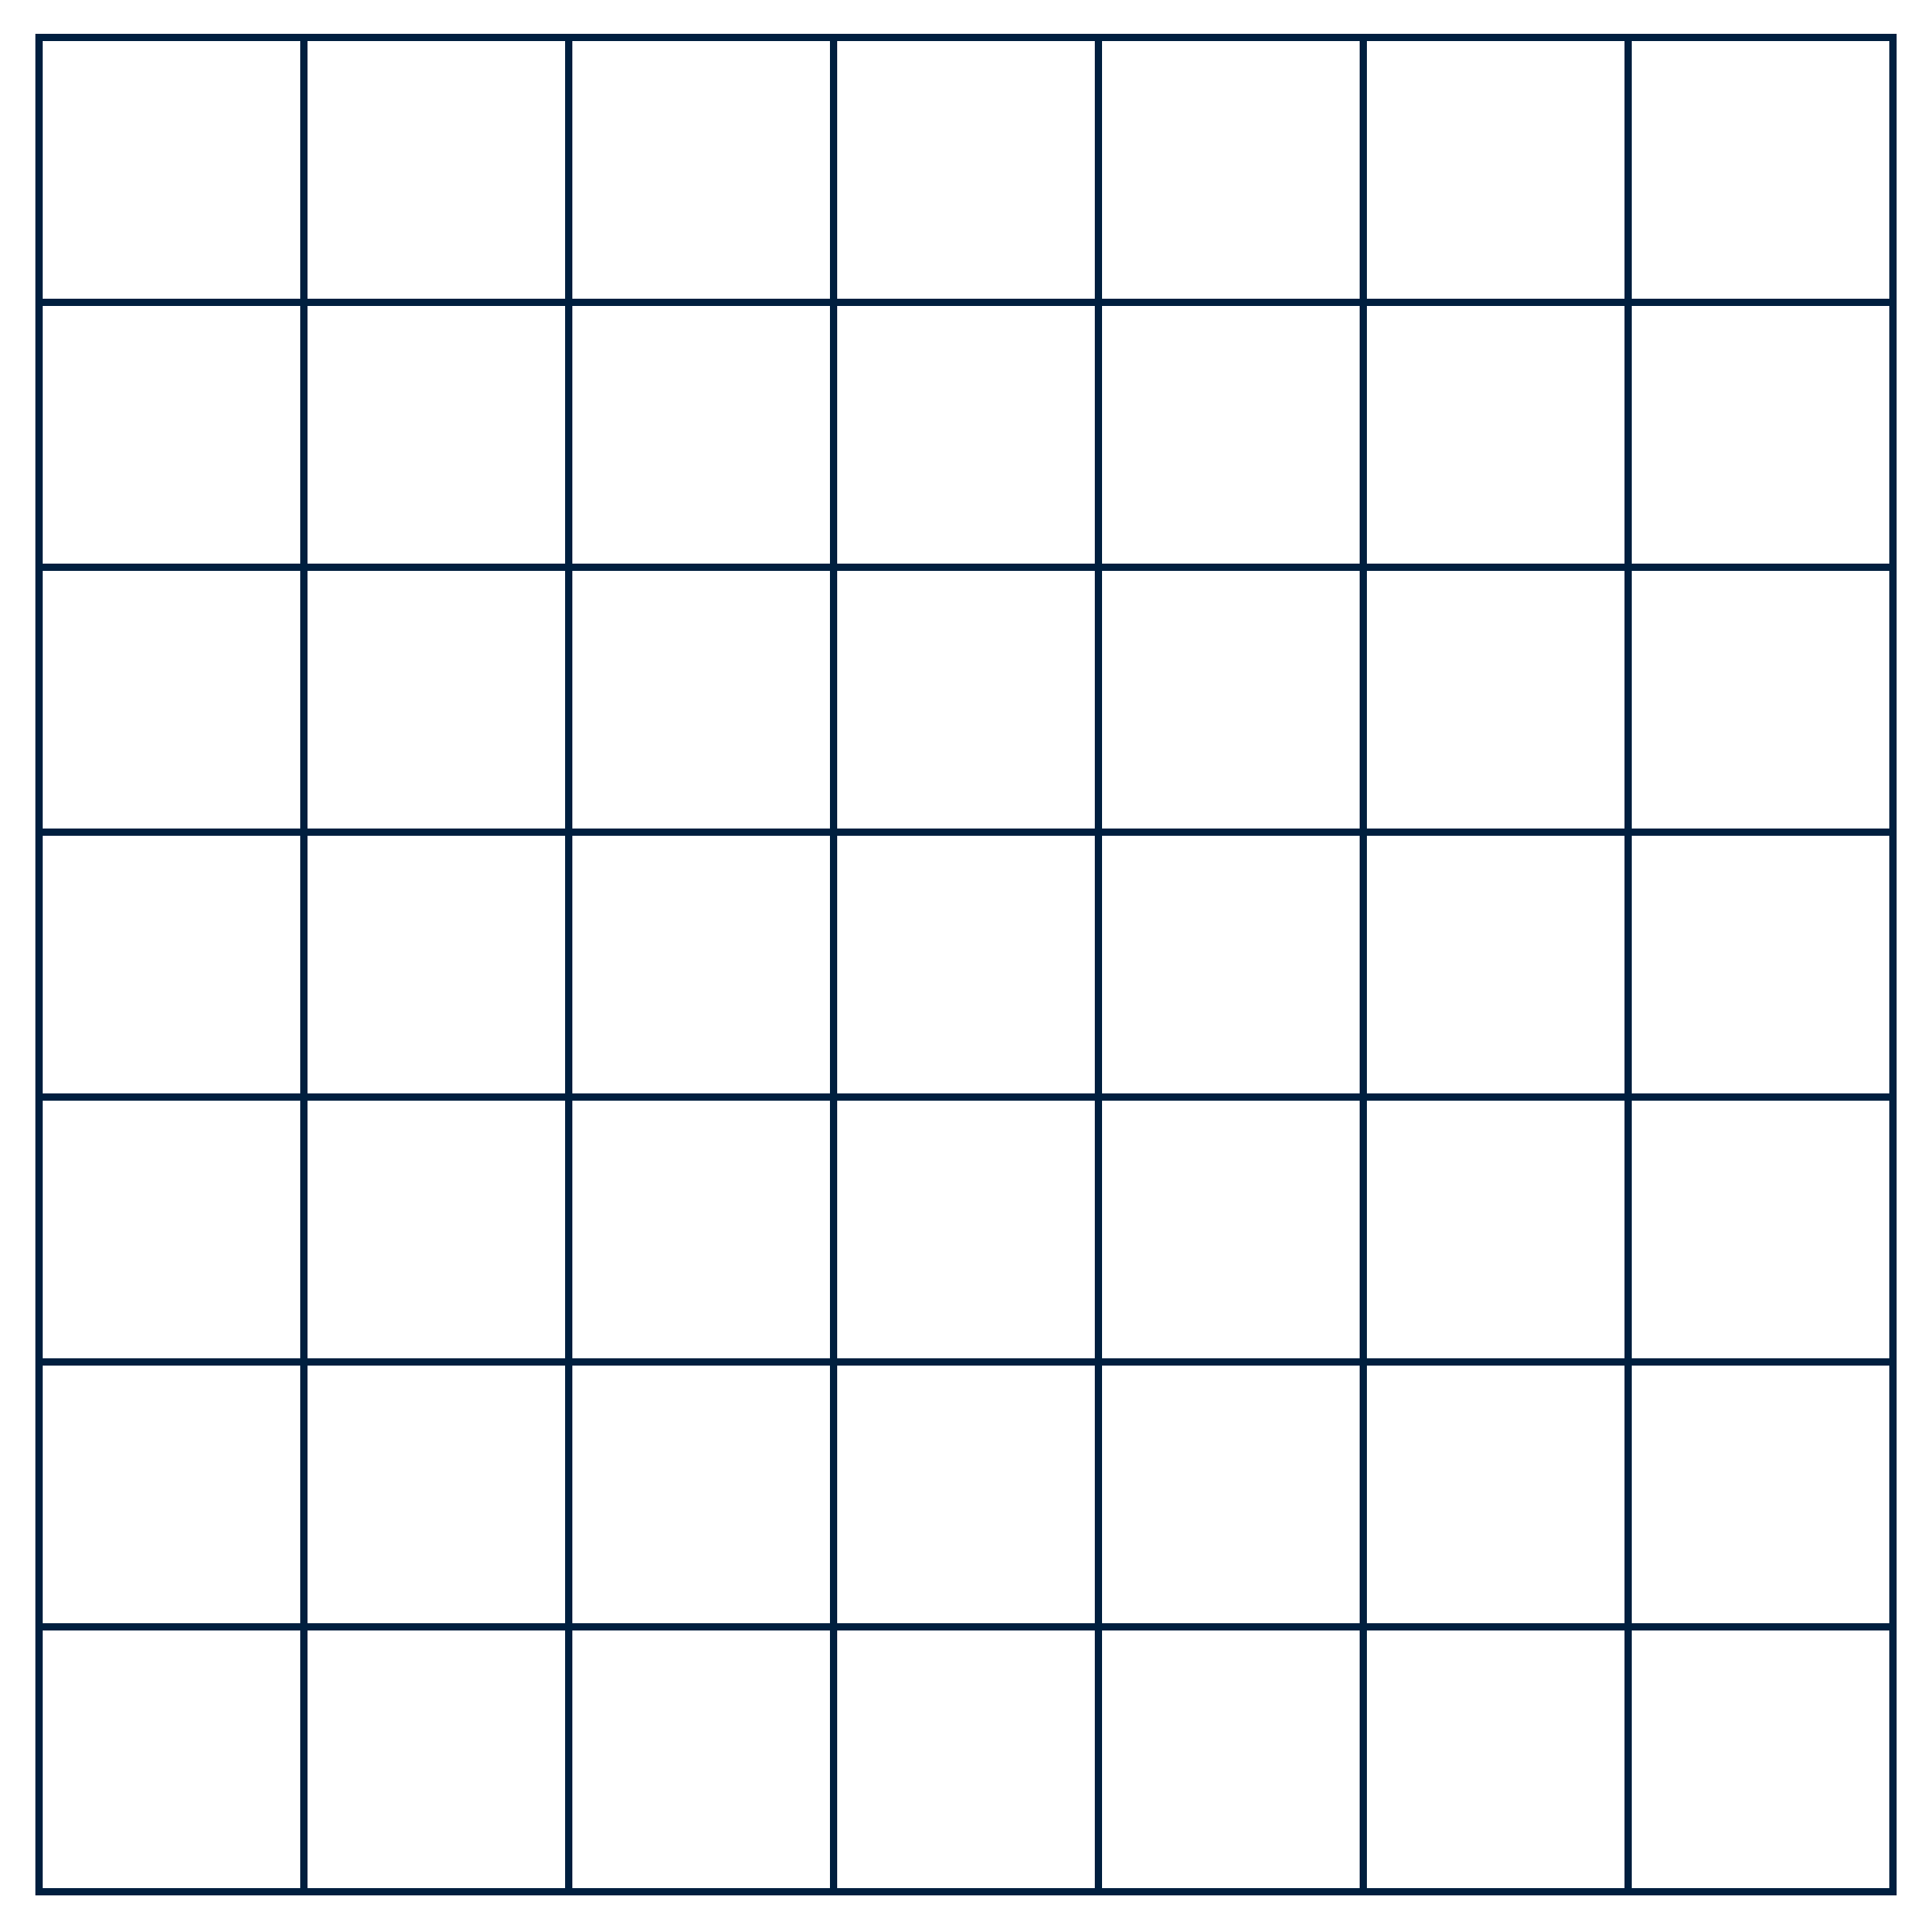
\includegraphics[width=\textwidth]{square}
                \caption{Tiling by squares}
                \label{fig:square}
        \end{subfigure}
        ~ %add desired spacing between images, e. g. ~, \quad, \qquad, \hfill etc.
          %(or a blank line to force the subfigure onto a new line)
        \begin{subfigure}[hb]{0.3\textwidth}
                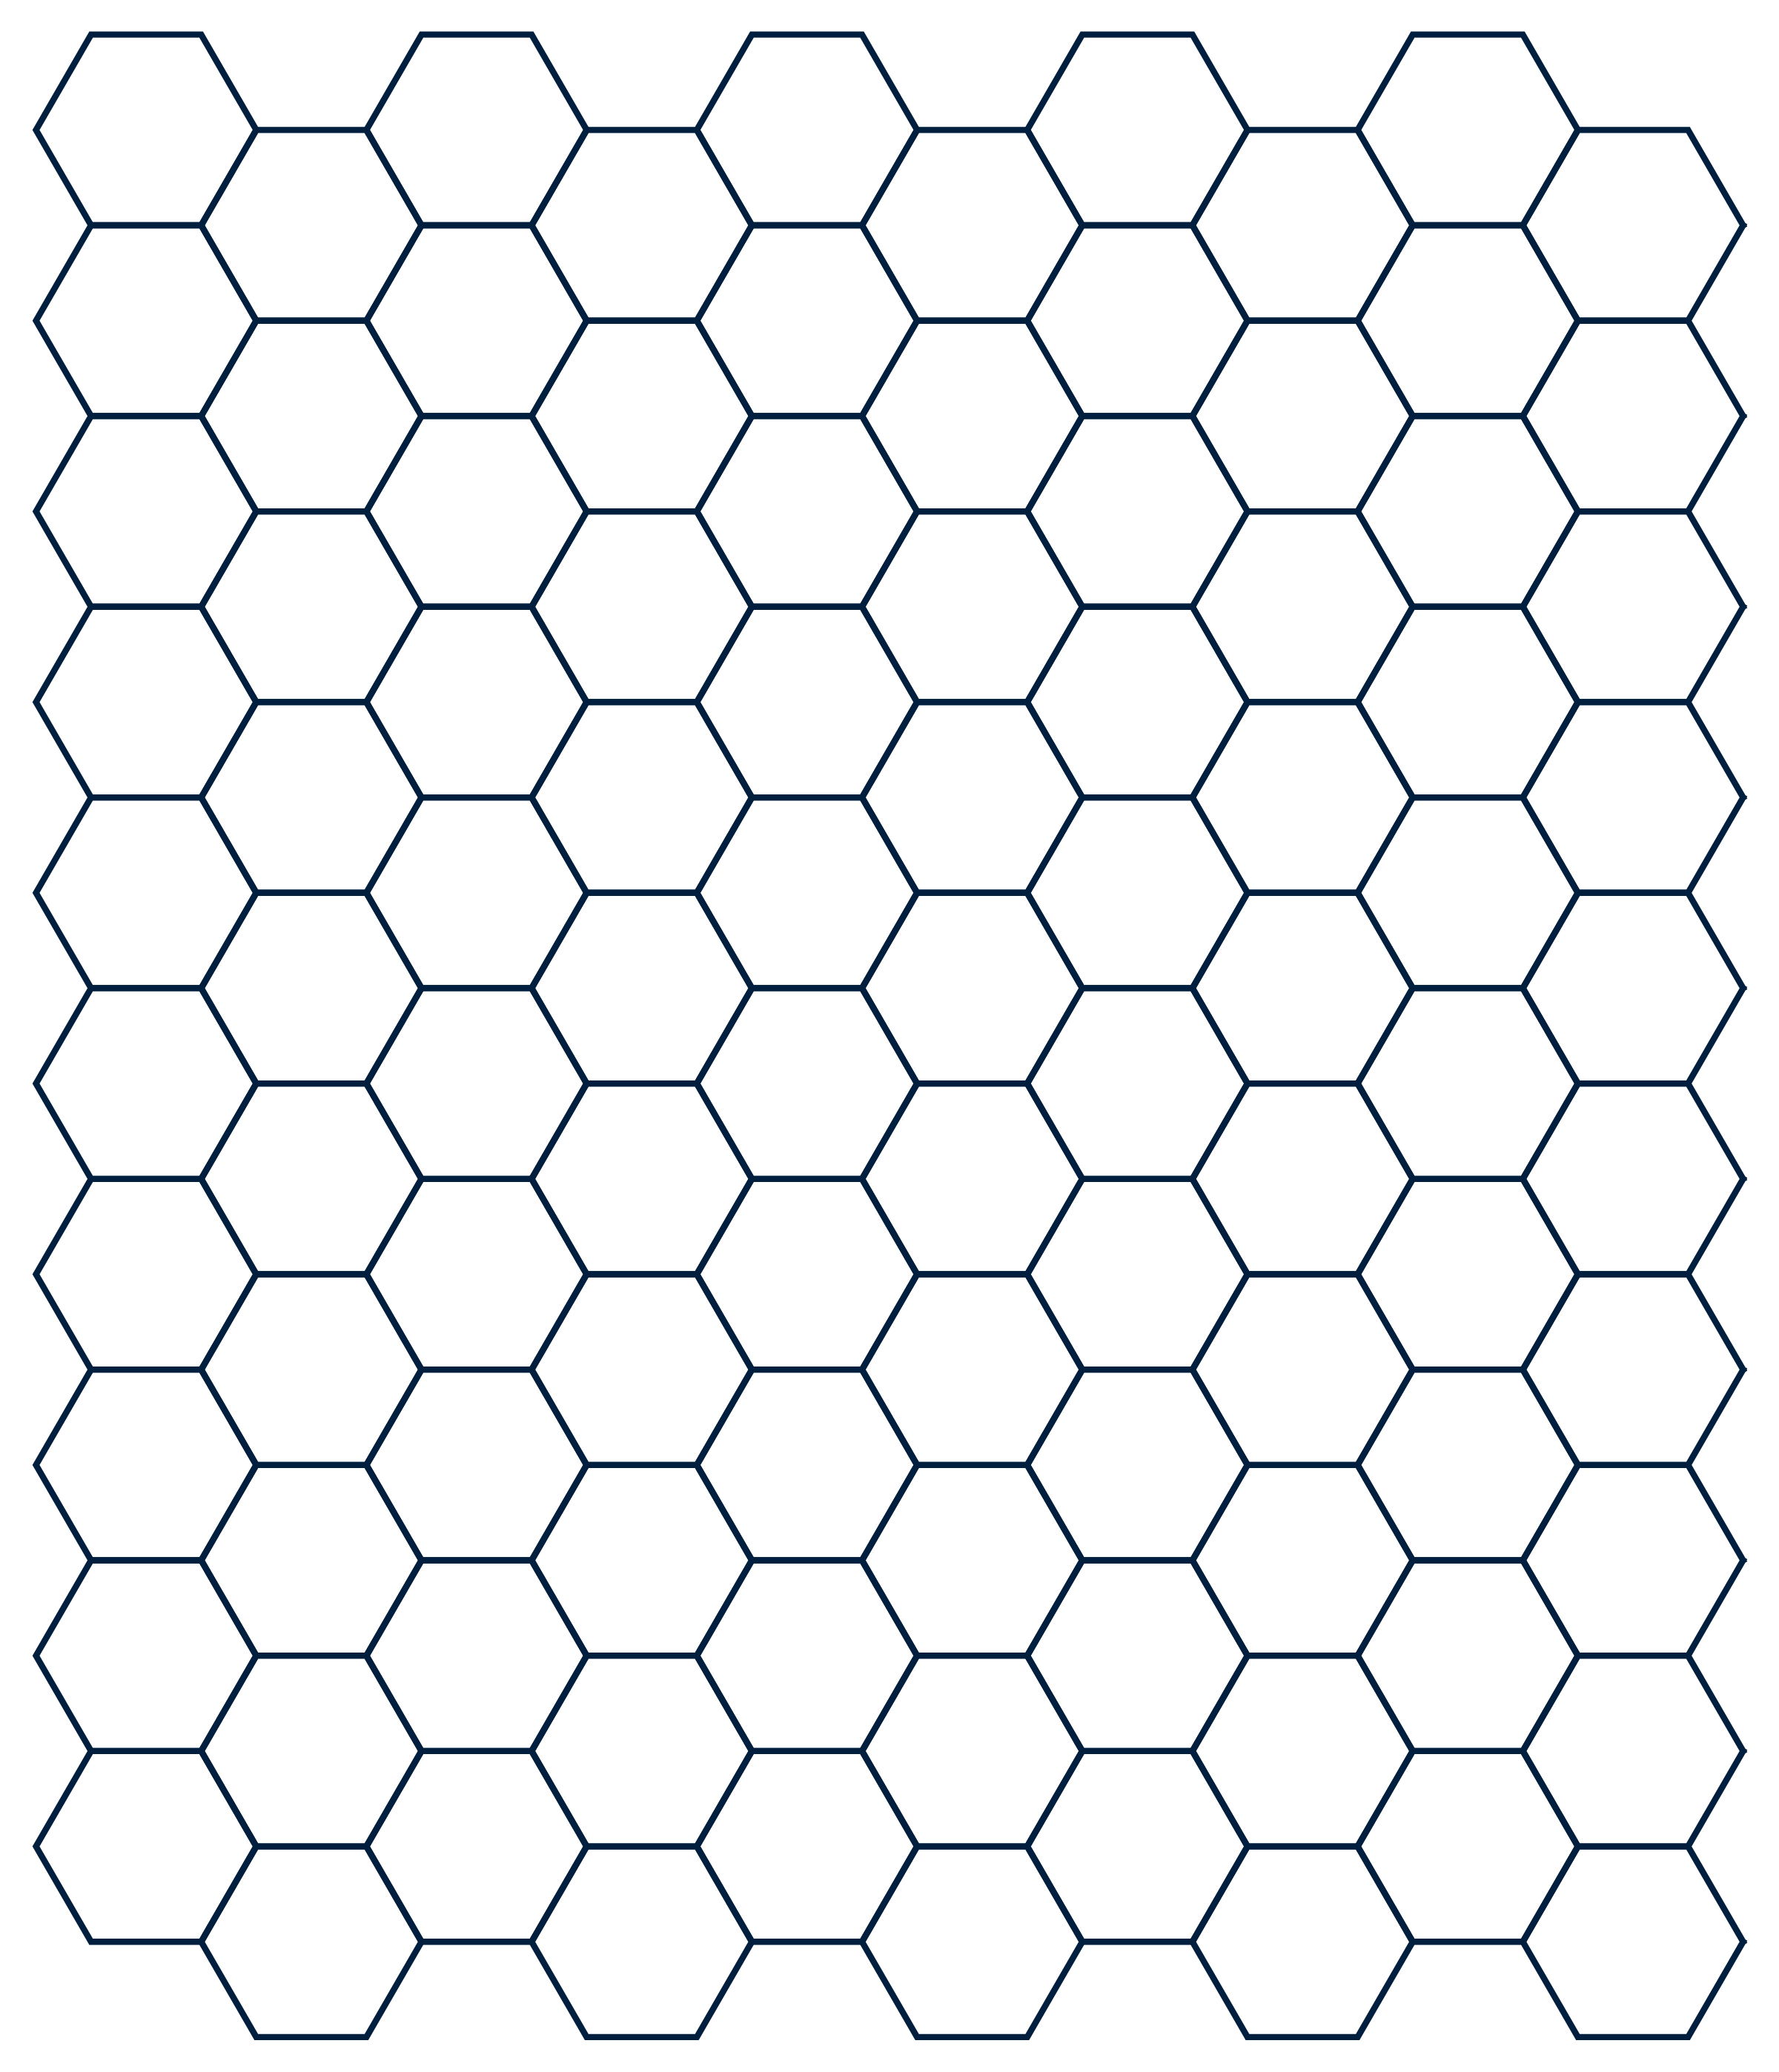
\includegraphics[width=\textwidth]{hexagon}
                \caption{Tiling by hexagons}
                \label{fig:hexagon}
        \end{subfigure}
        \caption{Regular tiling of the plane using single polygons}\label{fig:regular}
\end{figure}

\begin{figure}
        \centering
        \begin{subfigure}[hb]{0.3\textwidth}
                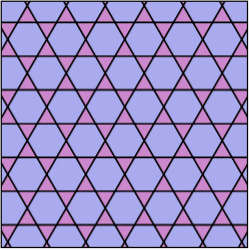
\includegraphics[width=\textwidth]{trihexagon}
                \caption{Trihexagonal }
                \label{fig:trihex}
        \end{subfigure}%
        ~ %add desired spacing between images, e. g. ~, \quad, \qquad, \hfill etc.
          %(or a blank line to force the subfigure onto a new line)
        \begin{subfigure}[hb]{0.3\textwidth}
                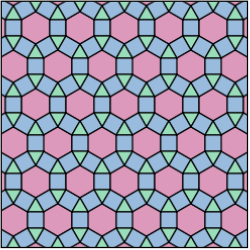
\includegraphics[width=\textwidth]{rhombitrihexagon}
                \caption{Rhombitrihexagonal}
                \label{fig:rhombitri}
        \end{subfigure}
        ~ %add desired spacing between images, e. g. ~, \quad, \qquad, \hfill etc.
          %(or a blank line to force the subfigure onto a new line)
        \begin{subfigure}[hb]{0.3\textwidth}
                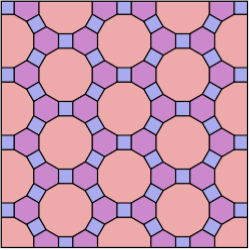
\includegraphics[width=\textwidth]{truncatedtrihexagon}
                \caption{Truncated trihexagon \textbf{}}
                \label{fig:trunctrihexagon}
        \end{subfigure}
        \caption{Periodic tiling of the plane using combination of polygons}\label{fig:combo}
\end{figure}

\subsection{History of Aperiodic Tiling}
We've seen that square tiles can be used to produce both periodic and aperiodic tiling, depending on the rules used to tile. This is also true for the triangles of Fig. \ref{fig:triangle}. However, the hexagons of Fig. \ref{fig:hexagon} cannot be arranged to tile aperiodically. Think of these hexagons as 'locked in' to each other, and unlike the squares and triangles there is no way to jostle the tiles into an aperiodic pattern. So squares and triangles can create both periodic and aperiodic tilings, but patterns using only hexagon tiles must be periodic. Of course, as seen in Fig. \ref{fig:combo}, we can make patterns with sets of multiple tiles which force periodicity like the hexagons (Fig. \ref{fig:trunctrihexagon}) or may allow both periodic and aperiodic tiling (consider Fig. \ref{fig:trihex} randomly jostled diagonally). This may lead you to a logical following question, are there a set of tiles which, when used to tile a plane, must be arranged aperiodically? In 1966, Robert Berger found a set of such tiles that force their tiling to be aperiodic, though his set required 20,426 tiles! Later, Berger was able to reduce the number of required tiles to 104. An even smaller set of six aperiodic tiles was discovered in 1971 by Raphael M. Robinson. Finally, Roger Penrose in 1973 reduced the required number of tiles to two! Any tiling from the two Penrose tiles, darts and kites, will be aperiodic.



\subsection{Definitions}
We will begin our discussion of Penrose tilings with some definitions given by Senechal \cite{Senechal1996}. First, a formal definition of a tiling of Euclidean n-space, $\mathbb{E}^n$:



\begin{mydef}
A \textbf{tiling} $\mathcal{T}$ of the space $\mathbb{E}^n$ is a countable family of closed sets, $T$, called tiles:
\begin{equation*}
\mathcal{T}=\{T_1,T_2,\mathellipsis\}
\end{equation*}
such that
\begin{enumerate}
\item $\mathcal{T}$ has no overlaps: $\mathring{T_i} \cap \mathring{T_j}=\emptyset$ if $i\neq j$
\item $\mathcal{T}$ has no gaps: $\bigcup_{i=1}^\infty T_i = \mathbb{E}^n$
\end{enumerate}
\end{mydef}


Here $\mathring{T}$ denotes the interior of tile $T$. Further, we assume that a tile is the closure of its interior, and that tiles have positive volume. These assumptions allow, for example, a line segment to be a tile in $\mathbb{E}^1$ but not in $\mathbb{E}^2$. Notice that this definition of tiling neither restricts the shape of the individual tiles nor the number of unique tiling shapes.  

However, we will impose some restrictions on the tiles here. Since we are considering tilings of the plane, our tiling must satisfy the above definition for $n=2$, that is, for the Euclidean plane $\mathbb{E}^2$. Further, while the general definition does not impose any criteria on tile shape, for our purposes we will only consider n-dimensional polytopes. In the case of the plane, we consider only 2-polytopes, or polygons. To denote the facets of our tiles we will use \textbf{edges} to denote the 1-dimensional faces, and \textbf{vertices} to denote the 0-dimensional faces. 

\begin{mydef}
Let $\{T_1,T_2,\mathellipsis\}$ be the set of tiles of tiling $\mathcal{T}$, partitioned into a set of equivalence classes by criterion $\mathcal{M}$. The set, $\mathcal{P}$, of representatives of these equivalence classes is called the \textbf{protoset} for $\mathcal{T}$ with respect to $\mathcal{M}$.
\end{mydef}

For example, consider an infinite black-and-white checkerboard (Fig.\ref{fig:checkerboard}). Each tile in the checkerboard is either a black or white square, and the tiling is given by the matching rule that black squares may only share edges with white squares, and vice-versa. In this example, the equivalence class criterion, $\mathcal{M}$, is the colour of the square together with this matching rule. The protoset, $\mathcal{P}$, for the checkerboard is the set containing two elements: a black square and a white square.

\begin{figure}[H]

  \hspace*{\fill}
\begin{subfigure}[t]{0.4\textwidth}
	\includegraphics[width=\textwidth]{Checkerboard}
    \caption{Checkerboard}
    \label{fig:checkerboard}
\end{subfigure}
  \hspace*{\fill}
\begin{subfigure}[t]{0.4\textwidth}
	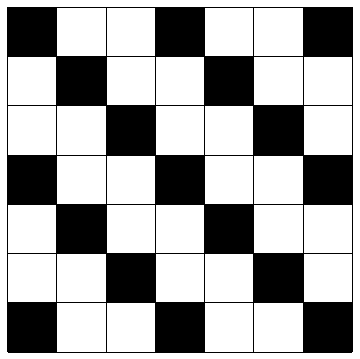
\includegraphics[width=\textwidth]{CheckerboardOther}
    \caption{Different Criterion.}
    \label{fig:critchecker}
\end{subfigure}
  \hspace*{\fill}\\
  \hspace*{\fill}
  \begin{subfigure}[t]{0.4\textwidth}
  	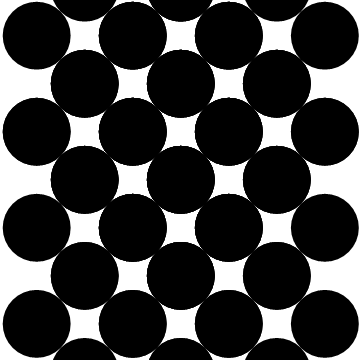
\includegraphics[width=\textwidth]{CheckerboardCircles}
      \caption{Deformed Checkerboard}
      \label{fig:deformedchecker}
  \end{subfigure}
      \hspace*{\fill} 
\begin{subfigure}[t]{0.4\textwidth}
	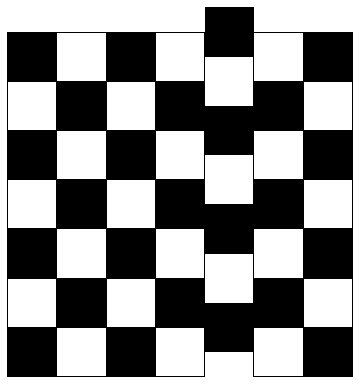
\includegraphics[width=\textwidth]{CheckerboardAperiodic}
    \caption{Sub-Periodic Checkerboard}
    \label{fig:aperiodicchecker}
\end{subfigure} 
\hspace*{\fill}
\label{fig:checker}
\caption{A protoset of black and white squares can admit multiple tilings. Some of them may be periodic, but this is not necessary.}
\end{figure}

\begin{mydef}
If $\mathcal{T}$ is a tiling with protoset $\mathcal{P}$, then we say that $\mathcal{P}$ admits $\mathcal{T}$.
\end{mydef}

In the checkerboard example we say that the protoset containing black and white squares, together with the matching criterion, admits a checkerboard tiling (Fig.\ref{fig:checkerboard}). It is important to note that a protoset can admit multiple tilings given different criterion. For example, the checkerboard protoset also admits the tiling in Fig.\ref{fig:critchecker} under a different matching rule. 

Further, it is also worth noting that abstract criterion, such as colour-matching or directed edges, can be accomplished instead through deformation of the edges of protoset tiles such that the criterion is forced. Consider again the criterion for producing the checkerboard tiling (Fig.\ref{fig:checkerboard}), that black squares may only share edges with white squares, and vice-versa. One way to realize this criterion is to deform all black squares into circles, and to deform white squares into curved diamonds. As seen in Fig.\ref{fig:deformedchecker}, these deformations force a tiling such that all white tiles occupy the interstices of the black circles. In other words, the protoset of deformed tiles, the black circle and white curved diamond, can only admit one unique tiling. We are able to force a checkerboard patter without any abstract criterion such as colour-matching adjacent tiles. While it is important to understand that abstract matching criterion can be realized by edge deformations, considering simpler protosets with more complicated criterion will usually allow greater insight into the structure and patterns within a tiling than would considering a simple criterion with complicated prototiles. 

\begin{mydef}
A tiling of  $\mathbb{E}^n$ is said to be \textbf{periodic} if it admits translational symmetry in $n$ linearly independent directions.
\end{mydef}

For example, the checkerboard tiling in Fig.\ref{fig:checkerboard} is periodic, as it has translational symmetry in two directions: vertical translation by two units, and horizontal translation by two units. Likewise, we can see that the criterion generating Fig.\ref{fig:critchecker} produces a tiling which is also periodic, with vertical and horizontal translational symmetry given by translation by three units. 

\begin{mydef}
A tiling of  $\mathbb{E}^n$ is said to be \textbf{sub-periodic} if it admits translational symmetry in $k$ linearly independent directions, where $1\leq k\leq n$. A tiling is said to be \textbf{non-periodic} if it admits no translational symmetry. 
\end{mydef}

For example, consider the checkerboard pattern with a single `column' translated vertically by a half-unit distance (Fig.\ref{fig:aperiodicchecker}). This tiling admits translational symmetry in the vertical direction with translation by two units. However, we can see that there is no horizontal symmetry because horizontal translation will not allow the shifted column to overlap anywhere. For this reason, there are also no diagonal translational symmetries admitted. This column shifted checkerboard is sub-periodic. 

We've seen that the protoset of black and white squares admits multiple types of tiling, both periodic and sub-periodic. Some protosets, such as the circle and curved diamond (Fig.\ref{fig:deformedchecker}), admits tilings which are only periodic. A question which motivated the discovery of the Penrose tiles was whether we can find protosets that admit \textit{only} non-periodic tilings.

\begin{mydef}
A protoset $\mathcal{P}$ is said to be \textbf{aperiodic} if it admits only non-periodic tilings. A tiling $\mathcal{T}$ from an aperiodic protoset is called an \textbf{aperiodic tiling}. 
\end{mydef}


\subsection{The Forbidden Symmetry}


\begin{mythm}
No tiling can have more than one center of fivefold rotational symmetry.
\label{symthm}
\end{mythm}

\begin{figure}[H]
	\centering
	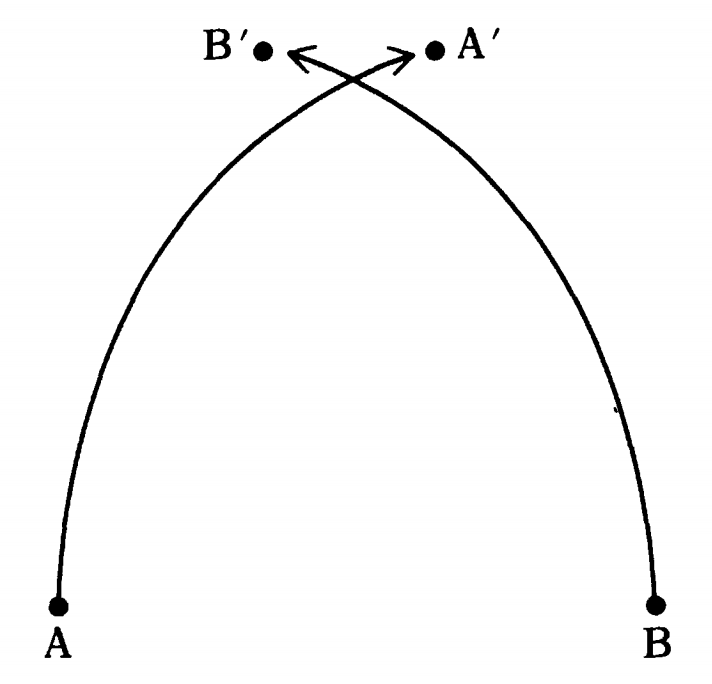
\includegraphics[width=0.4\textwidth]{proof}
    \caption{Barlow's Proof that no tiling can have more than one center of fivefold symmetry.}
    \label{fig:fivefoldproof}
\end{figure}

Conway provides a proof of this, attributed to Peter Barlow \cite{Gardner1997}.

\begin{proof}
Suppose in order to derive a contradiction that a tiling $\mathcal{T}$ has more than one center of fivefold symmetry.\\
Choose two centers, A and B, such that they are the nearest possible centers. \\
Rotate $\mathcal{T}$ counter-clockwise by $\frac{2\pi}{5}$ about $A$, bringing $B$ to $B'$, (see Fig.\ref{fig:fivefoldproof}).\\
Rotate $\mathcal{T}$ clockwise by $\frac{2\pi}{5}$ about $B$, bringing $A$ to $A'$.\\
A and B are centers of fivefold symmetry, so the tiling will overlap identically.\\
$\implies$ $A'$ and $B'$ are centers of fivefold symmetry.\\
But $A'$ and $B'$ are closer than $A$ and $B$.\\
This contradicts hypothesis that $A$ and $B$ are nearest centers of fivefold symmetry.\\
$\therefore$ By contradiction, $\mathcal{T}$ can only have one center of fivefold symmetry.
\end{proof}

We've shown that no tiling can have more than one center of fivefold symmetry. Using this theorem we can show, further, that even one center of fivefold symmetry is impossible if the tiling is periodic. First, consider these properties of periodic tilings:

\begin{myprop}
A periodic tiling can be subdivided into countably infinitely many regions, $\mathcal{R}$, which are congruent by translation such that
\begin{enumerate}
\item Two regions have no common interior points: $\mathring{\mathcal{R}_i} \cap  \mathring{\mathcal{R}_j}=\emptyset$ if $i\neq j$
\item The union of regions is exactly the tiling: $\bigcup_{i=1}^\infty \mathcal{R}_i = \mathcal{T}=\mathbb{E}^n$
\item For any two regions, $\mathcal{R}_i$ and $\mathcal{R}_j$, there is a translation that takes  $\mathcal{R}_i$ to $\mathcal{R}_j$. This translation also admits symmetry, carrying the entire tiling onto itself. \label{periodprop3}
\end{enumerate}
\label{periodprop}
\end{myprop}

\begin{mylem}
If tiling $\mathcal{T}$ is periodic, then it cannot have any centers of fivefold symmetry.
\end{mylem}
The proof of this is identical to the proof of Theorem \ref{symthm}.
\begin{proof}
Suppose in order to derive a contradiction that A is a center of fivefold rotational symmetry.\\
Since $\mathcal{T}$ is periodic, by condition \ref{periodprop3} of Property \ref{periodprop}, we see that there must be countably infinitely many centers of fivefold symmetry.\\
By Theorem \ref{symthm}, this is impossible.\\
$\therefore$ By contradiction, periodic tilings have no centers of fivefold symmetry.
\end{proof}

We have shown that fivefold symmetry is incompatible with periodic tilings. For this reason, the admittance of a single center fivefold symmetry is related to the aperiodicity of a tiling. As we will see, centers of fivefold symmetry are possible in Penrose tilings. 

\nocite{Penrose1979,Ogawa1999,Kepler1997,DeBruijn1990,DeBruijn1989,DeBruijn1981,Conway1986}
\bibliographystyle{plain}
\bibliography{bibliography}



\end{document}



Proof of no fivefold symmetry
Substitution Construction
Projective Construction
Up-Down Construction
Pentagrid

